\documentclass[11pt,a4paper]{report}
\usepackage[utf8]{inputenc}
\usepackage[french]{babel}
\usepackage[T1]{fontenc}
\usepackage{amsmath}
\usepackage{amsfonts}
\usepackage{amssymb}
\usepackage{xcolor}
\usepackage{gensymb}

\usepackage{geometry}
\geometry{hmargin=2.5cm,vmargin=1.5cm}
\usepackage{wasysym}
\usepackage{graphicx}

\author{Mathieu Sarrat}
\title{LP21 - Absorption et émission de la lumière}

\makeatletter
\renewcommand{\thesection}{\@arabic\c@section}
\makeatother


\begin{document}
\maketitle

\section*{Pré-requis, objectifs}
\subsubsection*{Niveau : Licence}

\subsubsection*{Pré-requis}
\begin{itemize}
	\item Rayonnement du corps noir
	\item Corde vibrante
	\item Interférences
	\item Oscillateurs quasi-sinusoïdaux en électronique
\end{itemize}

\subsubsection*{Recommandations :}
\begin{itemize}
	\item La démo du 1.2 n'est pas au programme de prépa, les relations entre coefficients d'Einstein 			sont admises. Ne pas faire le calcul (gain de temps), juste expliquer les hypothèses.
\end{itemize}
\newpage
\section*{Introduction}

Parmi les rares "nuages" venant obscurcir le "ciel bleu" de la physique à la fin du $\text{XIX}^\text{e}$ siècle (pour paraphraser Lord Kelvin) se trouvait la catastrophe ultraviolette : selon la théorie classique, le corps noir est censé émettre des rayonnements toujours plus importants à mesure que la longueur d'onde diminue, ce qui n'est pas conforme aux résultats expérimentaux. Pire, ce modèle prédit une énergie rayonnée infinie.

Planck, en supposant la discrétisation des échanges d'énergie entre le rayonnement électromagnétique et la matière, résolut ce problème. ceux-ci se faisant par l'intermédiaire de petits paquets d'énergie (quantas) tels que
\begin{equation}
	\Delta E = h \nu,
\end{equation}
$\nu$ désignant la fréquence de l'onde électromagnétique échangeant son énergie avec le milieu environnant.

Einstein va plus loin en proposant que l'énergie, et pas seulement les échanges, sont quantifiés.

\newpage
\section{Modèle des probabilités de transition}

Nous allons discuter le modèle proposé par Einstein, en 1917, pour décrire les processus d'émission et d'absorption de lumière.

\subsection{Processus d'interaction lumière-matière}

\subsubsection{Position du problème}

Le système étudié se compose :
\begin{itemize}
	\item d'un rayonnement, de \textbf{densité volumique spectrale d'énergie} $w(\omega)$,
	qui peut être du rayonnement thermique ou un rayonnement électromagnétique autre.
	\item d'atomes, modélisés par un \textbf{système à deux niveaux d'énergie} $E_1 < E_2$. Seules des 		fréquences voisines de $\nu_0$, telle que
	\begin{equation}
		\boxed{E_2 - E_1 = h\nu_0}	
	\end{equation}
	ont une probabilité non-négligeable d'interagir avec le système. Les deux niveaux d'énergie sont 		supposés \textbf{non-dégénérés} (1 niveau correspond à 1 état).\\
\end{itemize}

Soient $N$ atomes par unité de volume, dont $N_1$ dans le niveau 1 et $N_2$ dans le niveau 2 :
\begin{equation}
	\boxed{N = N_1 + N_2 = \text{cte}}.\\
\end{equation}

Pendant une durée dt, ces atomes peuvent subir une transition (du niveau 1 vers le niveau 2 ou vice-versa) sous l'effet d'un processus d'interaction lumière-matière. Einstein propose 3 processus élémentaires : \textbf{émission spontanée, émission stimulée, absorption}.\\

Le nombre d'atomes subissant une transition suite à un même type de processus s'écrit :
\begin{equation}
	\boxed{dN_\text{processus} = \pm N p_\text{processus} dt}
\end{equation}
Il y a proportionnalité à la durée considérée et au nombre d'atomes pouvant transiter. $p_\text{processus}$ désigne une \textbf{probabilité par unité de temps}.

\subsubsection{Absorption}

Le système dans l'état d'énergie $E_1$ peut absorber un photon d'énergie $h\nu_0$, pour atteindre le niveau d'énergie $E_2$. C'est le \textbf{phénomène d'absorption} :
\begin{equation}
	\boxed{\left(\frac{dN_1}{dt} \right)_\text{abs.} = - p_\text{abs.}N_1 = - w(\omega_0)B_{12}N_1}.
\end{equation}
\begin{figure}[h!]
\begin{center}
	\begin{tabular}{cc}
		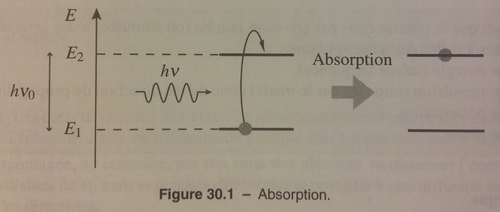
\includegraphics[scale = 0.55]{absorption.png}
	\end{tabular}
\end{center}
\caption{Absorption.}
\end{figure}
La probabilité par unité de temps dépend de la densité spectrale d'énergie volumique, car il faut bien un rayonnement à absorber pour qu'il y ait absorption. Le coefficient $B_{12}$ est appelé \textbf{coefficient d'Einstein pour l'absorption}.

\subsubsection{Émission stimulée}
Le système se trouve dans l'état excité d'énergie $E_2$. Le champ électromagnétique présent peut provoquer la désexcitation vers le niveau 1 et induire l'émission d'un photon d'énergie $h\nu_0$, pourvu qu'il existe de l'énergie électromagnétique à la fréquence $\nu_0$.
\begin{equation}
	\boxed{\left(\frac{dN_2}{dt} \right)_\text{stim.} = - w(\omega_0)B_{21}N_2}.
\end{equation}
\begin{figure}[h!]
\begin{center}
	\begin{tabular}{cc}
		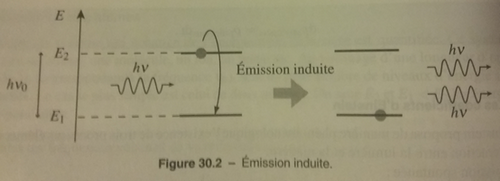
\includegraphics[scale = 0.55]{stimulee.png}
	\end{tabular}
\end{center}
\caption{Émission stimulée.}
\end{figure}

Le photon émis a même fréquence, même direction de propagation (même quantité de mouvement), même polarisation et même phase que les autres photons émis par émission stimulée. Là encore, la probabilité par unité de temps dépend de la densité spectrale d'énergie volumique puisque c'est le rayonnement déjà présent qui induit l'émission. Le coefficient $B_{21}$ est appelé \textbf{coefficient d'Einstein pour l'émission stimulée}. 

\subsubsection{Émission spontanée}
Le système se trouve dans l'état excité d'énergie $E_2$. On s'attend intuitivement à ce que cet état ne perdure pas et que le système revienne spontanément au niveau 1, en émettant un photon d'énergie $h\nu_0$.
\begin{equation}
	\boxed{\left(\frac{dN_2}{dt} \right)_\text{spont.} = - A_{21} N_1}.
\end{equation}
\begin{figure}[h!]
\begin{center}
	\begin{tabular}{cc}
		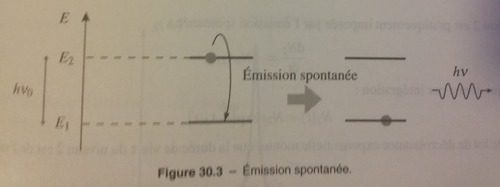
\includegraphics[scale = 0.55]{spontanee.png}
	\end{tabular}
\end{center}
\caption{Émission spontanée.}
\end{figure}

Ce processus est indépendant de la présence d'un rayonnement ambiant. On suppose une probabilité par unité de temps constante : le coefficient $A_{21} = p_\text{spont.}$ est appelé \textbf{coefficient d'Einstein pour l'émission spontanée}. La population $N_2(t)$ décroit selon
\begin{equation}
	N_2(t) = N_{20}\text{e}^{-\text{A}_{21}t}
\end{equation}
en l'absence d'émission stimulée et d'absorption, faisant de $\Delta\tau = 1/\text{A}_{21}$ \textbf{la durée de vie typique du niveau excité}. Le photon émis par émission spontanée a une direction de propagation aléatoire, une polarisation et une phase aléatoire, ainsi qu'une \textbf{fréquence aléatoire, mais voisine} de $\nu_0$. Alors pourquoi voisine ?
 
\subsubsection{Profils de raie}

On a toujours supposé que seuls des photons de fréquence
\begin{equation}
	\nu_0 = \frac{E_2 - E_1}{h},
\end{equation}
pouvaient interagir avec les atomes. Ceci suppose que les énergies $E_1$ et $E_2$ soient bien définies, c'est à dire que les deux états considérés soient des états stationnaires. En pratique, ils ne le sont pas, car la relation d'incertitude d'Heisenberg implique :
\begin{equation}
	\Delta \tau \Delta E \geq \frac{\hbar}{2}.
\end{equation}
Si les niveaux d'énergie sont stationnaires $\Delta E = 0$, donc $\Delta \tau \rightarrow \infty$ : \textbf{le niveau excité, s'il est stationnaire, a une durée de vie infinie, prohibant toute désexcitation spontanée}.\\

Comme l'émission spontanée existe
\begin{equation}
	\boxed{\Delta E = h\Delta \nu \neq 0}
\end{equation}
et, en reprenant la relation d'Heisenberg,
\begin{equation}
	\boxed{\delta \nu \simeq \text{A}_{21}}.
\end{equation}
traduisant une certaine \textbf{tolérance sur la fréquence des photons} pouvant interagir avec le système.\\

Cette \textbf{largeur spectrale naturelle} est de l'ordre de 1 à 100 MHz, ce qui est très faible devant les fréquences typiques du rayonnement visible ($\simeq$ 500 THz).\\

Il existe d'autres sources d'élargissement spectral :
\begin{itemize}
	\item \textbf{l'effet Doppler}, lié au mouvement des atomes émetteurs ou absorbants par rapport à 			l'observateur :
		\begin{equation}
			\nu_\text{reçue} = \nu_\text{émise}\left(1 - \frac{v}{c} \right)
		\end{equation}
		pour un déplacement selon l'axe reliant l'atome et l'observateur. L'effet Doppler conduit à des 		largeurs spectrales de l'ordre du GHz, masquant généralement la largeur naturelle.
	\item \textbf{les collisions}, les chocs entre atomes provoquent des sauts de phase : la vibration 			émise n'est pas sinusoïdale, et le modèle des trains d'ondes permet par exemple d'en tenir 				compte. L'élargissement collisionnel est important dans un gaz dense.\\
\end{itemize}

\begin{figure}[h!]
\begin{center}
	\begin{tabular}{cc}
		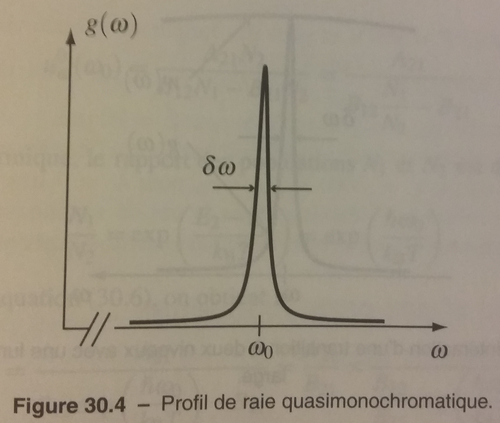
\includegraphics[scale = 0.45]{profilderaie.png}
	\end{tabular}
\end{center}
\caption{Profil de raie quasimonochromatique.}
\end{figure}

Pour quantifier ces effets, on habille la raie spectrale monochromatique d'un \textbf{profil de raie}, fonction notée $g(\omega)$, centrée sur $\omega_0 = 2\pi\nu_0$ et de largeur à mi-hauteur $\delta\omega$ telle que
\begin{equation}
	\delta \omega \ll \omega_0 \quad\text{et}\quad \int_0^{+\infty} g(\omega)d\omega = 1.
\end{equation}
Cette fonction vient pondérer les probabilités de transition, par exemple pour l'émission stimulée
\begin{equation}
	p_\text{stim.} = B_{21}\int_0^\infty g(\omega)w(\omega)d\omega \simeq B_{21}w(\omega_0)
\end{equation}
pour un rayonnement de \textbf{spectre large} interagissant avec les atomes. C'est dans cette approximation que nous avons écrit les probabilités par unité de temps des trois processus présentés plus haut.

\newpage
\subsection{Équilibre rayonnement atomes}
\subsubsection{Bilan de population}
Comme $N = N_1 + N_2$ est constante,
\begin{equation}
	\frac{dN_1}{dt} = - \frac{dN_2}{dt} \quad\text{d'où}\quad
	\boxed{\frac{dN_2}{dt} = w(\omega_0)\left(B_{12} N_1 - B_{21}N_2\right) - A_{21}N_2}.
\end{equation}

\subsubsection{Relations entre coefficients d'Einstein}
On suppose un rayonnement à spectre large interagissant avec la transition 12, et un ensemble d'atomes à l'équilibre thermodynamique avec ce rayonnement. Ce rayonnement est de type corps noir, donc de densité spectrale d'énergie volumique $w(\omega_0)$ donnée par la \textbf{Loi de Planck} (vérifiée expérimentalement) :
\begin{equation}
	w(\omega_0) = \frac{\hbar \omega_0^3}{\pi^2 c^3}
	\frac{1}{\displaystyle{\text{exp}\left(\frac{\hbar \omega_0}{k_B T}\right)-1}}.
\end{equation}
On montre qu'à l'équilibre
\begin{equation}
	\boxed{\frac{A_{21}}{B_{21}} = \frac{\hbar\omega_0^3}{\pi^2 c^3}} 
	\quad\text{et}\quad \boxed{B_{12} = B_{21}}.
\end{equation}
On doit maintenant faire plusieurs remarques :
\begin{itemize}
	\item Si on connaît un coefficient d'Einstein, on connaît les trois.
	\item Une théorie pleinement quantique des atomes et du champ électromagnétique fait apparaître 			naturellement ces coefficients, ainsi que les relations entre eux.
\end{itemize}

\subsubsection{Comparaison des processus d'émission}
\begin{equation}
	\frac{p_\text{stim.}}{p_\text{spont.}} = \frac{w(\omega_0)B_{21}}{A_{21}} 
	= \frac{1}{\displaystyle{\text{exp}\left(\frac{\hbar\omega_0}{k_B T}\right)-1}}
\end{equation}

\begin{itemize}
	\item T = 300K, pour le visible $\text{exp}\left(\frac{\hbar\omega_0}{k_B T}\right) \gg 1$, 
	donc $p_\text{stim.} \ll p_\text{spont.}$, donc l'émission spontanée domine. On a 
	$p_\text{stim.} \simeq p_\text{spont.}$ si $\lambda \simeq 70 \mu m$.;
	\item T = 3000K, si $\lambda \simeq 7 \mu m$ on a $p_\text{stim.} \simeq p_\text{spont.}$, et
	l'émission spontanée domine dans le visible.
\end{itemize}

\newpage
\section{Bilan de puissance}

\subsection{Bilan de puissance}

Soit un milieu constitué d'atomes dans l'état 1 ou dans l'état 2, parcouru par un rayonnement de pulsation $\omega$ sous forme d'onde plane. Faisons un bilan d'énergie et écrivons l'équation de conservation de l'énergie électromagnétique 
\begin{equation}
	\boxed{\frac{\partial w}{\partial t} + \text{div}\;\bold{R} 
	= \pi_\text{émis} - \pi_\text{abs.} - \pi_\text{pertes}},
\end{equation}
où $\bold{R}$ désigne une densité spectrale de puissance surfacique et où les termes sources décrivent 
\begin{itemize}
	\item la puissance spectrale volumique $(W/Hz)$ émise par les atomes du milieu
		\begin{equation}
			\pi_\text{émis} = -\hbar\omega \left[ \left(\frac{dN_2}{dt}\right)_\text{spont.}   
			+  \left(\frac{dN_2}{dt}\right)_\text{stim.} \right]
			= \left[A_{21} + B_{21}w(\omega)\right]N_2 g(\omega) \hbar\omega
		\end{equation}
	\item la puissance spectrale volumique absorbée par les atomes du milieu
		\begin{equation}
			\pi_\text{abs.} = -\hbar\omega \left(\frac{dN_1}{dt}\right)_\text{abs.}   
			= B_{12} N_1 w(\omega) g(\omega)\hbar\omega
		\end{equation}
	\item la puissance spectrale volumique perdue $\pi_\text{pertes}$ autrement que par absorption 				(\textcolor{red}{par exemple par diffusion ?})
\end{itemize}
Les profils de raies apparaissent car on ne suppose pas un rayonnement à spectre large. Pour simplifier l'étude, on va négliger l'émission spontanée et les pertes "autres", puis supposer un milieu unidimensionnel pour faire un bilan sur une tranche de milieu comprise entre l'abscisse z et l'abscisse z $+$ dz. On utilise $B_{12} = B_{21}$, d'où
\begin{equation}
	\frac{\partial w}{\partial t} + \frac{\partial R_z}{\partial z}
	= \left(N_2 - N_1\right)B_{12}w(\omega)g(\omega)\hbar\omega.
\end{equation}
En milieu dilué ($n = 1$), on a $R = wc$ (où $c$ désigne la vitesse de la lumière) d'où
\begin{equation}
	\frac{\partial w}{\partial t} + \frac{\partial R_z}{\partial z}
	= \left(N_2 - N_1\right)B_{12}g(\omega)\frac{\hbar\omega}{c}R_z,
\end{equation}
d'où
\begin{equation}
	\boxed{\frac{1}{c}\frac{\partial R_z}{\partial t} + \frac{\partial R_z}{\partial z} 
	= \gamma(\omega)R_z}
\end{equation}
où
\begin{equation}
	\boxed{\gamma(\omega) \equiv \left(N_2 - N_1\right)B_{12}g(\omega)\frac{\hbar\omega}{c}}
\end{equation}
désigne le \textbf{gain par unité de longueur}.\\

Ainsi, en régime stationnaire,
\begin{equation}
	\boxed{R_z(z) = R_0 \text{e}^{\gamma(\omega)z}}.
\end{equation}
\begin{itemize}
	\item si $\gamma(\omega) > 0$, il y a amplification au fur et à mesure qu'on se déplace dans le 			milieu. Mais cela n'est possible que si $N_2 > N_1$.
	\item si $\gamma(\omega) < 0$, ce qui correspond à $N_1 < N_2$, il y a absorption et donc perte de 			puissance dans le milieu.
\end{itemize}

\`A l'équilibre thermodynamique avec un thermostat de température $T$, la statistique de Maxwell-Boltzmann impose
\begin{equation}
	\frac{N_2}{N_1} = \text{e}^{-\frac{E_2 - E_1}{k_B T}},
\end{equation}
or $E_2 > E_1$, donc $N_1 > N_2$ et donc $\gamma(\omega) < 0$. Le \textbf{milieu est donc atténuateur à l'équilibre}.

\newpage
\subsection{Loi de Beer-Lambert}

Cette décroissance exponentielle de la puissance surfacique de l'onde électromagnétique nous rappelle la loi de Beer-Lambert, rencontrée assez fréquemment en chimie lors des dosages spectrophotométriques : En régiment permanent, le module du vecteur de Poynting s'identifie à l'intensité lumineuse (sinon c'est la moyenne du module) :
\begin{equation}
	I(z) = I_0 \text{e}^{\gamma(\omega)z} = I_0 \text{e}^{-|\gamma(\omega)|z}
\end{equation}

On définit l'\textbf{absorbance}, grandeur sans unité, comme
\begin{equation}
	A \equiv -\text{log}_{10}\frac{I(z)}{I_0}, 
\end{equation}
de sorte qu'on ait la loi de Beer-Lambert
\begin{equation}
	A = \epsilon [i] z,
\end{equation}
où $[i]$ désigne la concentration molaire en espèce absorbante et $\epsilon$ est un coefficient d'extinction molaire, proportionnel au gain défini précédemment.\\

On se propose de vérifier la dépendance linéaire de l'absorbance par rapport à l'épaisseur du milieu traversé par un rayonnement :
\begin{itemize}
	\item présenter le montage,
	\item prendre un point de mesure pour chaque épaisseur de matériau,
	\item comparer avec les résultats obtenus en préparation.
\end{itemize}

\subsubsection*{Interprétation probabiliste}

On reprend le bilan de population
\begin{equation}
	\frac{dN_1}{dt} = - \frac{dN_2}{dt} \quad\text{d'où}\quad
	\boxed{\frac{dN_2}{dt} = w(\omega_0)\left(B_{12} N_1 - B_{21}N_2\right) - A_{21}N_2}.
\end{equation}
et on fait une analyse dimensionnelle. On montre que
\begin{equation}
	[B] = \text{M}^{-1}\text{L},
\end{equation}
et donc que la quantité
\begin{equation}
	\boxed{\sigma \equiv B_{12}g(\omega) \frac{\hbar \omega}{c}}
\end{equation}
est homogène à une surface : c'est la \textbf{section efficace d'absorption}.

Un photon du rayonnement se déplace au milieu d'une assemblée d'atomes susceptibles de l'absorber. La probabilité $\mathcal{P}$ qu'à le photon d'être absorbé dans un volume cylindrique de section $S$ et de longueur $z$ \textcolor{red}{(faire un putain de schéma !)} est proportionnelle au nombre d'atomes $NSz$ contenus dans ce volume multiplié par le rapport $\sigma/S$, d'où
\begin{equation}
	\mathcal{P} = NSz \frac{\sigma}{S} = N \sigma z.
\end{equation}
Le \textbf{gain par unité de longueur peut donc s'interpréter comme une probabilité d'interaction} (absorption ou émission selon le signe de $\gamma$) \textbf{par unité de longueur}.

\newpage
\subsection{Amplification d'un signal}

Peut-on amplifier un rayonnement ? Nous avons vu deux problèmes :\\

\begin{itemize}
	\item Premièrement, à l'équilibre il y a davantage d'atomes susceptibles d'absorber que d'atomes 			susceptibles d'émettre. Il faut réaliser une \textbf{inversion de population} pour favoriser 			l'émission et amplifier le rayonnement. Un procédé utilisé est le \textbf{pompage optique}, 			inventé par Alfred Kastler. On peuple un niveau d'énergie $E_3$ supérieur au niveau $E_2$, qui 			est alors peuplé par les atomes effectuant une transition du niveau 3 vers le niveau 2. Il faut 		que le taux de peuplement du niveau 2 soit supérieur à son taux de désexcitation.\\
		
	\item Deuxièmement, l'émission spontanée produit un rayonnement constitué de photons dont les 				caractéristiques sont aléatoires (phase, quantité de mouvement, direction, polarisation), 				contrairement à l'émission stimulée qui produit des photons identiques. Si on veut amplifier un 		rayonnement, il faut que l'émission stimulée domine l'émission spontanée. Or, ce n'est qu'à des 		températures bien plus élevées que la valeur ambiante que l'émission stimulée domine dans le 			visible.\\ 
\end{itemize}

Nous avons vu en électronique des systèmes capables d'amplifier du bruit pour générer un signal quasi-sinusoïdal d'amplitude nettement supérieure au bruit qui lui a donné naissance. Ces oscillateurs quasi-sinusoïdaux sont des \textbf{systèmes bouclés}, utilisant le principe d'une rétroaction positive pour amplifier le signal initial, combiné à un filtre qui vient sélectionner la ou les composantes spectrales que l'on souhaite amplifier. Un exemple d'oscillateur quasi-sinusoïdal est l'oscillateur à pont de Wien (\textcolor{red}{Diapo !}) :\\
\begin{itemize}
	\item le montage amplificateur non-inverseur amplifie le signal d'entrée;
	\item le filtre de Wien est un filtre \textbf{passe bande} qui atténue toutes les composantes 				spectrales du signal, mais certaines sont moins atténuées que d'autres (celles situées autour 			de la fréquence de résonance de ce filtre passe-bande) Son gain maximal en amplitude est de 1/3 		pour la fréquence de résonance; 
	\item Le signal en sortie du pont de Wien est bouclé vers l'amplificateur, repasse par le 				filtre et ainsi de suite.\\
\end{itemize}

Une analyse électrocinétique de ce système conduit à l'équation différentielle suivante :
\begin{equation}
	\boxed{\frac{d^2r}{dt^2} + \frac{3-G}{RC}\frac{dr}{dt} + \frac{r}{(RC)^2} = 0},
\end{equation}
où l'on reconnaît l'expression d'un oscillateur de pulsation $\omega_0 = {1}/{RC}$ et de taux d'amortissement (au sens large) $RC/(3-G)$ avec $G = (R_1 + R_2)/R_1$ le gain de l'amplificateur non-inverseur. Lorsque $\omega = \omega_0$, le gain du filtre de Wien est maximal et égal à 1/3.\\
	
\textbf{La valeur de G détermine le comportement du système.} On peut contrôler la valeur de G en faisant varier une des deux résistances du montage non-inverseur (par exemple $R_2$) :\\
\begin{itemize}
	\item $G < 3$, les oscillations sont amorties et donc $r(t) \rightarrow 0$ : on ne récupère que du 			bruit en sortie : le gain de l'ampli ne suffit pas à compenser l'atténuation du filtre.
	\item $G > 3$, l'amplificateur amplifie plus que le filtre n'atténue, il y a donc instabilité et 			donc $r(t) \rightarrow +\infty$. En réalité, le signal finit par saturer sous l'effet de 				phénomènes non-linéaires (qui ne sont évidemment pas pris en compte dans notre modèle 					linéaire). La saturation est liée à l'amplificateur opérationnel, incapable de délivrer plus 			que sa tension de saturation (environ 15 V). Plus $G$ est élevé, plus on perd le caractère 				sinusoïdal du signal.
	\item $G = 3 \Leftrightarrow R_2 = 2R_1$, le gain de l'amplificateur compense exactement 					l'atténuation du filtre et le système se comporte comme un oscillateur harmonique de fréquence 			$f_0 = 1/(2\pi RC)$, entièrement déterminée par le pont de Wien. 
\end{itemize}

\begin{figure}[h!]
\begin{center}
	\begin{tabular}{cc}
		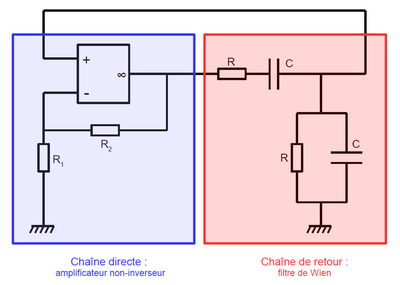
\includegraphics[scale = 0.6]{wien1.png} &
		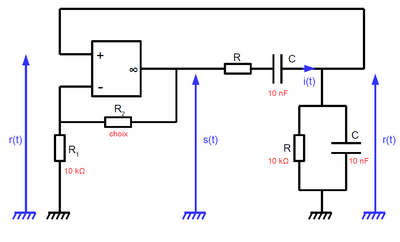
\includegraphics[scale = 0.6]{wien2.png} \\
	\end{tabular}
\end{center}
\caption{Oscillateur à pont de Wien.}
\end{figure}

\newpage
\section{Le LASER}

Le LASER (ou Light Amplification by Stimulated Emission of Radiation) est un \textbf{oscillateur optique} amplificateur de lumière. De façon schématique, il est constitué d'un milieu amplificateur de lumière (par exemple un gaz, comme dans le laser Hélium-Néon utilisé en TP) placé dans une cavité réfléchissante (par exemple deux miroirs, dans le cas d'une cavité rectiligne).

\begin{figure}[h!]
\begin{center}
		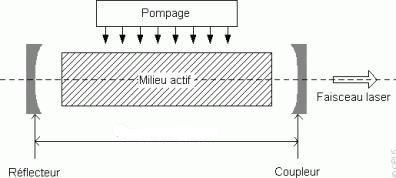
\includegraphics[scale = 1]{cavite2.png}
\end{center}
\caption{Principe du laser.}
\end{figure}

Ce système est un système bouclé, et pour y voir plus clair on peut construire une analogie avec l'oscillateur à pont de Wien :
\begin{itemize}
	\item le mécanisme d'amplification est l'émission stimulée (analogie avec l'AO non-inverseur);
	\item le bouclage est réalisé par les miroirs réfléchissants d'une cavité optique : l'onde 					électromagnétique subit des réflexions qui l'obligent à parcourir la cavité à de nombreuses 			reprises;
	\item la sélectivité en fréquence est la conséquence de phénomènes d'interférences;
	\item le bruit sur lequel démarre l'oscillateur est constitué des photons émis par émission 				spontanée.
\end{itemize}

\subsection{Cavité optique}

La cavité optique que nous venons de montrer est analogue à un interféromètre de Fabry-Pérot. Le miroir M1 est conçu pour avoir une réflectivité en énergie de 99\% alors que le miroir de sortie M2 en a une inférieure, de l'ordre de 95\%, permettant ainsi à une partie du faisceau de s'échapper du milieu amplificateur.\\

En première approximation, \textbf{supposons que les miroirs sont des conducteurs parfaits} de sorte que le champ électrique à leur surface soit nul. Une telle situation rappelle fortement le problème de la corde tendue, fixée à ses deux extrémités. On peut montrer que les solutions stationnaires (c'est à dire les modes propres) de l'équation de d'Alembert ont la forme
\begin{equation}
	\Psi(z,t) = \text{sin}(\omega_p t)\text{sin}(k_p z)
\end{equation}
où
\begin{equation}
	k_p = p\frac{\pi}{L}, 
\end{equation}
où $p$ est un entier. On peut réécrire cette condition comme
\begin{equation}
	\frac{2L}{\lambda_p} = p.
\end{equation}
Tous les modes ne peuvent pas se développer dans une telle cavité.\\

On peut interpréter cette condition en termes d'interférences d'ondes planes : soit une onde progressive se réfléchissant indéfiniment sur les miroirs. La différence de phase accumulée après un aller retour est
\begin{equation}
	\Delta\Phi = \frac{2\pi}{\lambda_p}2L = 2\pi \text{p},
\end{equation}
$p$ étant un entier. Cela implique que toute onde de longueur d'onde $\lambda_p$ est en phase avec elle-même après un aller-retour : il y a interférences constructives. Les ondes dont les longueurs d'ondes diffèrent de $\lambda_p$ vont interférer destructivement avec elles-mêmes et ne pourront pas se développer. C'est ce phénomène d'interférences qui est à l'origine de la sélectivité spectrale de la cavité optique.

\subsubsection{Pertes}

Parmi les causes de pertes d'énergie, on peut citer :
\begin{itemize}
	\item le fait que la réflectivité des miroirs ne soit pas totale.
	\item le fait qu'il y ait toujours de l'émission spontanée, de la lumière est émise dans toutes les 			directions.
	\item le fait qu'il y ait de la diffraction sur les miroirs, qui ont une taille finie.
\end{itemize}

\subsubsection{Accrochage et saturation du gain}

De manière analogue à l'oscillateur à pont de Wien, il y aura amplification (on parle d'accrochage) si le gain en énergie le long d'un aller dans la cavité surpasse les pertes accumulées. Cela permet à l'oscillateur de démarrer sur le bruit (constitué entre autres par l'émission spontanée).\\

L'amplitude lumineuse ne va pas croître jusqu'à l'infini, car l'émission stimulée va tendre à réduire l'inversion de population et donc à diminuer le gain. Cela va provoquer la saturation du phénomène.

\subsection{Fonctionnement en régime permanent}

\subsubsection*{Condition de fonctionnement}

En régiment permanent, on compense tout juste les pertes, tout comme l'oscillateur quasi-sinusoïdal à pont de Wien.

\subsubsection*{Fréquences émises par le laser}

Rappelons que le gain $\gamma(\omega)$ est proportionnel à $\omega g(\omega)$ où $g$ désigne un profil de raie, dont la largeur $\Delta \nu_D$ correspond typiquement à l'élargissement Doppler (environ 1 GHz). Les modes propres de la cavité de Fabry-Pérot sont séparés de
\begin{equation}
	\Delta \nu_c = \frac{c}{2nL},
\end{equation}
quantité appelée \textbf{intervalle spectral libre}, valant 500 MHz pour L $=$ 30cm et n $=$ 1. Le nombre de modes pour lesquels le gain est capable de compenser les pertes est donc réduit (grand maximum 3) avec les ordres de grandeur considérés. Un laser peut-être monomode si un seul mode est amplifié, multimode si plusieurs le sont.\\

\begin{figure}[h!]
\begin{center}
	\begin{tabular}{cc}
		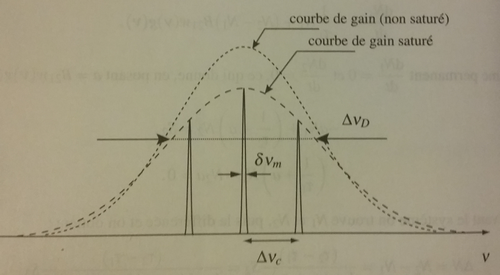
\includegraphics[scale = 0.45]{final.png}
	\end{tabular}
\end{center}
\caption{Modes émis par un laser : explication.}
\end{figure}

Enfin, les modes de la cavité de Fabry-Pérot ne sont pas rigoureusement monochromatiques. On attribue une largeur spectrale $\delta \nu_m$ à chaque pic, liée au facteur de qualité de la cavité. En première approximation, on considère que cette grandeur ne dépend que de la réflectivité \textbf{(coefficient de réflexion en énergie R)} des miroirs (0.95 pour le miroir de sortie et 0.99 pour l'autre dans le cas d'une cavité rectangulaire) ce qui conduit à une valeur de 8 MHz environ.\\

Pour le laser Hélium-Néon utilisé fréquemment en TP (L $=$ 30 cm, $\lambda = $ 633 nm, soit une fréquence d'environ $\nu \simeq$ 474 THz), l'entier $p$ est de l'ordre de $10^6$. Une faible variation de la longueur de la cavité est démultipliée et entraine des variations de fréquences non-négligeables :
\begin{equation}
	\Delta \nu = \frac{\nu}{L}\Delta L.
\end{equation}
Ainsi, la fréquence varie de $\Delta \nu_D =$ 1.5 GHz (largeur Doppler) pour une variation de longueur de la cavité d'environ 1 $\mu m$. On comprend qu'il soit compliqué d'avoir une fréquence stable, puisque le laser est soumis en permanence à des vibrations et à des fluctuations de température.

\subsubsection*{Puissance émise par le laser}
En régime permanent, lorsque l'émission stimulée résultant du pompage compense les pertes du laser, le gain est saturé, proportionnel à l'inversion de population
\begin{equation}
	\Delta N = N_2 - N_1 = \frac{\tau_2 - \tau_1}
	{1 + \left( \tau_1 + \tau_2 \right) \frac{B_{21}g(\omega)}{c}\mathcal{E}} S_2
\end{equation}
où $\mathcal{E}$ désigne l'éclairement (moyenne temporelle du module du vecteur de Poynting). La puissance dépend donc de la fréquence et du taux de pompage $S_2$.\\

Les ordres de grandeur de taille et de puissance sont variés. Le laser Hélium Néon utilisé typiquement en travaux pratiques a une longueur de 30 cm pour une puissance de quelques mW. Les lasers utilisés en ophtalmologie délivrent une puissance de quelques $\mu$W.

\section*{Conclusion}

Nous nous sommes surtout intéressés au régime permanent du fonctionnement d'un laser. Il existe cependant des lasers pulsés, capables aujourd'hui de délivrer des impulsions de quelques femtosecondes, voire attosecondes. Le laser PETAL (PETawatt Aquitaine Laser) aura une puissance de 1.2 PW, soit plus de $10^{15}$ W : il délivrera une énergie d'environ 1 kJ sur une impulsion d'une picoseconde. Le laser Mégajoule délivrera des impulsions d'environ 15 kJ sur 20 nanosecondes.\\

Les applications du rayonnement laser, continu comme pulsé, sont extrêmement nombreuses : 
\begin{itemize}
	\item vie quotidienne : pointeurs laser, effets visuels, travaux pratiques de physique;
	\item télémétrie, procédés industriels (découpage, gravure);
	\item médecine : dermatologie (effacement de tatouages), ophtalmologie (cataracte, myopie...);
	\item fusion thermonucléaire contrôlée : laser Mégajoule;
	\item astrophysique de laboratoire, pour générer des plasmas et reproduire à échelle miniature et 			de façon contrôlée des phénomènes lointains.
\end{itemize}



\newpage
\section*{Annexes}

\subsection*{Démonstration des relations entre coefficients d'Einstein}

\`A l'équilibre
\begin{equation}
	\frac{dN_2}{dt} = 0 \quad\text{d'où}\quad	
	0 = w(\omega_0)\left(B_{12} N_1 - B_{21}N_2\right) - A_{21}N_2
\end{equation}
et donc
\begin{equation}
	w(\omega_0) = \frac{\displaystyle{A_{21}}}{\displaystyle{B_{12}\frac{N_1}{N_2}-B_{21}}}.
\end{equation}

\`A l'équilibre, la statistique de Maxwell-Boltzmann implique
\begin{equation}
	\frac{N_1}{N_2} = \text{exp}\left(\frac{E_2-E_1}{k_B T}\right) 
	= \text{exp}\left(\frac{\hbar \omega_0}{k_B T}\right),
\end{equation}
d'où
\begin{equation}
	w(\omega_0) = \frac{A_{21}}{B_{21}}\frac{1}{\displaystyle{\frac{B_{12}}{B_{21}} \text{exp}\left(\frac{\hbar \omega_0}{k_B T}\right)-1}}.
\end{equation}

Par identification avec la Loi de Planck, on en déduit :
\begin{equation}
	\boxed{\frac{A_{21}}{B_{21}} = \frac{\hbar\omega_0^3}{\pi^2 c^3}} 
	\quad\text{et}\quad \boxed{B_{12} = B_{21}}
\end{equation}

\newpage
\subsection*{Expérience : absorption de la lumière blanche}

\subsubsection*{Matériel :}
	\begin{itemize}
	\item Diapo "Beer-Lambert" : épaisseurs e de calque/plastique multiples entiers d'une épaisseur 				"zéro", teintées au permanganate de potassium (ou autre colorant). Tracer A $=$ f(e)
	\item Lampe QI, condenseur, filtre anti-calorique, lentille de focale 150 ou 200 mm, banc 						d'optique, écran
	\item Spectromètre USB avec fibre optique et logiciel approprié.
	\end{itemize}

\subsubsection*{Protocole :}
	\begin{itemize}
	\item Banc d'optique : réaliser la conjugaison entre la diapo, placée sur un pied coulissant 				latéralement et l'écran par la lentille. Placer la diapo près de la lampe, intercaler le filtre 		anti-calorique si besoin. Régler le condenseur et la lampe pour former l'image du 						filament sur la lentille.
	\item Remplacer l'écran par la fibre optique et placer l'écran derrière (on peut ainsi savoir ce 			qu'observe la fibre).
	\item Sur Atelier Scientifique avec Spectro USB Spectrovio :
		\begin{itemize}
			\item Menu absorbance, tracer le spectre d'absorption, repérer une longueur d'onde où 								l'absorbance de la région la plus concentrée en colorant ne sature pas.
			\item Menu $A =f(x)$ : faire le blanc "Calibration" et suivre les instructions.
			\item Tracer la courbe en déplaçant latéralement la diapo.
			\item Faire une étude statistique (au moins 30 mesures sur une même tranche, en déplaçant 					la fibre optique sur toute la tranche. Éventuellement, demander au technicien de 						répéter les mesures sur les autres tranches.
		\end{itemize}		 
	\end{itemize} 
\end{document}